\documentclass[12pt]{ctexbeamer}

    %主题和色彩风格
    % http://latex.artikel-namsu.de/english/themes/uebersicht_beamer.html
    % \usetheme{metropolis}
    % \usetheme{Madrid}
    % \usetheme{Pittsburgh}
    % \usetheme{Copenhagen}
    % \usetheme{Boadilla}

    \usetheme{Frankfurt}
    \usecolortheme{orchid}

    \usefonttheme{serif}              % 使用衬线字体
    \usefonttheme{professionalfonts}  % 数学公式字体
    \usepackage{mathtools}

    % \usepackage{appendixnumberbeamer}
    % \usepackage{pdfpages}
    \usepackage{booktabs}
    % \usepackage[scale=2]{ccicons}

    % \usepackage{pgfplots}
    % \usepgfplotslibrary{dateplot}

    \usepackage{xspace}
    % \newcommand{\themename}{\textbf{\textsc{metropolis}}\xspace}

    \usepackage{multirow}

    \renewcommand {\thetable}{\thesection{}.\arabic{table}}
    \renewcommand {\thefigure}{\thesection{}.\arabic{figure}}

    \title{基于LightGBM分类的上市公司财务报表舞弊识别研究}
    % \subtitle{2020年毕业论文答辩}
    \date{}
    \author{答辩人: 会计1610王淙烨 \qquad \newline 指导老师: 孙景翠 \newline}
    % \institute{东北农业大学}
    % \titlegraphic{\hfill\includegraphics[height=1.5cm]{logo.pdf}}

\begin{document}

\maketitle

%%%%%%%%%%%%%%%%%%%%%%%%%%%%%%%%%%%%%%%%%%%%%%%%%%%%%%%%%%%%%%%
% 说明
%
% \section{}命令是分节
%
% \begin{frame}[fragile]{%此处添加标题} \end{frame}
%
% \begin{verbatim} 此处是中间凸出位置,可以放latex代码\end{verbatim}
%
% \href{网址}{文字}
%
% \emph{斜体}
%
% \begin{itemize}是无序列表
% \item <内容>
%%%%%%%%%%%%%%%%%%%%%%%%%%%%%%%%%%%%%%%%%%%%%%%%%%%%%%%%%%%%%%%

% 目录
\begin{frame}{目录}
    \setbeamertemplate{section in toc}[sections numbered]
    \tableofcontents[hideallsubsections]
  \end{frame}

% 设计目的与意义
\section{背景介绍}

\begin{frame}{研究背景}

    \begin{columns}[T,onlytextwidth]

        \column{0.3\textwidth}
            目的
            \begin{itemize}
                \item 定量分析
                \item 辅助判断
                \item 解释原因
            \end{itemize}

        \column{0.36\textwidth}
            意义
            \begin{itemize}
                \item 避免误导投资者
                \item 维护债权人利益
                \item 提高市场出清效率
            \end{itemize}
        \column{0.3\textwidth}
            创新点
            \begin{itemize}
                \item 样本容量大
                \item 解释变量多
                \item 模型效果好
            \end{itemize}

    \end{columns}

\end{frame}


% 论文结构和主要内容
\section{论文结构}

\begin{frame}[fragile]{论文结构}
    \begin{description}
        \item[第一部分] 前言
        \item[第二部分] 相关概念综述
        \item[第三部分] 样本选取与分析
        \item[第四部分] 财务舞弊识别分类器构建
        \item[第五部分] 结论
    \end{description}
\end{frame}


% 详细工作
\section{主要内容}


\begin{frame}[fragile]{样本结构}
    \begin{figure}
        \includegraphics[width=11cm]{Pic/样本审计意见分类图.png}
        \caption{审计意见分类}
    \end{figure}
\end{frame}

\begin{frame}[fragile]{样本结构}
    \begin{figure}
        \includegraphics[width=11cm]{Pic/样本比例.png}
        \caption{各行业比例}
    \end{figure}
\end{frame}

\begin{frame}[fragile]{样本结构}
    \begin{figure}
        \includegraphics[width=11cm]{Pic/样本中非标准意见分布.png}
        \caption{非标准意见分布}
    \end{figure}
\end{frame}

\begin{frame}[fragile]{模型结构}
    \begin{figure}
        \includegraphics[width=10cm]{Pic/模型结构.pdf}
        \caption{模型结构}
    \end{figure}
\end{frame}

\begin{frame}[fragile]{模型评价}
    \begin{table}[]
        \caption{模型判别预测准确率}
        \begin{tabular}{ccccc}
        \toprule
        \multirow{3}{*}{观测值}  & \multicolumn{4}{c}{预测类型}                                     \\ \cline{2-5}
                                & \multicolumn{3}{c}{异常类型}          & \multirow{2}{*}{准确率(\%)} \\ \cline{2-4}
                                &           & $Y_{i}=0$ & $Y_{i}=1$ &                          \\ \hline
        \multirow{2}{*}{异常类型} & $Y_{i}=0$ & TP=28947  & FP=0      & 100                      \\
                                & $Y_{i}=1$ & FN=14     & TN=977    & 98.59                    \\ \cline{1-2}
        \multicolumn{2}{c}{整体准确率}         & TPR=99.95 & FPR=0     & 99.95                    \\ \bottomrule
        \end{tabular}
        \end{table}
\end{frame}

\begin{frame}[fragile]{模型评价}
    $$ACC=\frac{TP+TN}{P+N}=99.95\%$$
    $$PRE=\frac{TP}{TP+FP}=100\%$$
    $$REC=\frac{TP}{TP+FN}=98.59\%$$
    $$F_{1}-Score=\frac{2}{\frac{1}{PRE}\frac{1}{REC}}=99.47\%$$
\end{frame}

\begin{frame}[fragile]{模型评价}
    \begin{figure}
        \includegraphics[width=10cm]{Pic/ROC_AUC.png}
        \caption{ROC-AUC曲线}
    \end{figure}
\end{frame}

\begin{frame}[fragile]{变量分析}
    \begin{figure}
        \includegraphics[width=11cm]{Pic/均值降低精度.png}
        \caption{均值降低精度}
    \end{figure}
\end{frame}

\begin{frame}[fragile]{变量分析}
    \begin{figure}
        \includegraphics[width=11cm]{Pic/特征重要性排序.png}
        \caption{特征重要性排序}
    \end{figure}
\end{frame}

\begin{frame}[fragile]{变量分析}
    \begin{figure}
        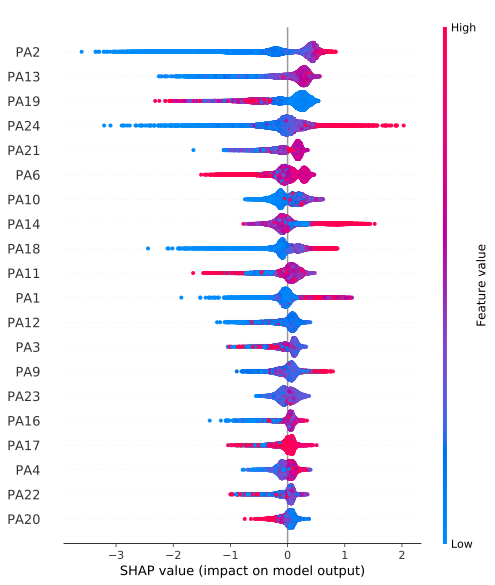
\includegraphics[width=5cm]{Pic/shap_summary.png}
        \caption{特征Shap值分布}
    \end{figure}
\end{frame}


% 结论
\section{结论}

\begin{frame}{结论}
    \begin{itemize}
        \item 舞弊强行业聚集性
        \item 企业现金流\&每股息税前利润
        \item 模型简单\&识别效果好
    \end{itemize}
\end{frame}


% 结语
\section*{致谢}

\begin{frame}
        \begin{center}
                \Huge{\textbf{谢 \quad 谢}}
        \end{center}
\end{frame}


\end{document}